\chapter{Methods}
    \label{cha:methods}
    %
    \section{Chromatin Model}
    \label{sec:ChromatinModel}
        %
        The chromatin in \ed/ is modelled as an array of half-nucleosomes (for simplicity, the array of half-nucleosomes  is referred to as nucleosome string in the rest of the work), meaning that they only contain one tetramer of H2A, H2B, H3 and H4. The nucleosomes hold their respective position on the string so that the neighbour relations are fixed. That way, every nucleosome has exactly two neighbouring nucleosomes (in the cyclic case, see below) that stay the same throughout the entirety of a simulation. Furthermore, the nucleosomes are reduced to presence or absence of PTMs on their tails.
        %

        %
        The model in this work can even be reduced further, so that a nucleosome is modelled as 1 ($K27$) single amino acid which can be either acetylated (referred to as active) or monomethylated (referred to as silenced). Di- and trimethylation will not be featured in this work. Exceptionally, in \ref{sec:ResBivalency}, every nucleosome possesses 2 modifiable amino acids, called $K_x$ and $K_y$. All of these amino acids are monoacetylatable as well as monomethylatable. These two modifications are mutually-exclusive one one amino acid. However, $K_x$ and $K_y$ can very well contain opposing modifications in which case the concerning nucleosome will be referred to as bivalent.\\
        %

        %
        The nucleosome string is either modelled to be non-cyclic (as done in \ref{sec:ResNon-cooperative} and \ref{sec:ResNonCyc}) or cyclic (\ref{sec:ResBistableSwitching} to \ref{sec:ResBivalency}). In the cyclic case, the enzymes' context can include nucleosomes from the start as well as the end of the string simultaneously. In the non-cyclic case, the first and last nucleosome logically only have one neighbour.
        %

        %
        The non-cyclic models contain 60 nucleosomes whereas the cyclic ones only contain 40 nucleosomes in order to reduce computation time and storage space.
        %

        %
        The starting state for every simulation in this work is a completely unmodified nucleosome string. As long as there are random adders in the system (which is the case for every system featured in this work), the completely unmodified string logically is an unstable configuration which does not offer any sort of bias in the direction of acetylation or methylation respectively, hence the choice of an entirely unmodified starting state. The time it takes the system to adjust to establishing a modified string is negligible compared to the total time of one simulation run.
        %
    %
    %
    \section{Enzyme models}
        %
        \subsection{Enzymes in \ed/}
            %
            The enzymes in \ed/ are mainly described by their reaction nature, the context needed in order to perform the reaction, their association and their dissociation rate. The reaction nature defines the change that the enzyme is performing on the nucleosomes' modifications. Generally, the enzymes are either modification adders or modification removers (see \ref{subsec:EnzymeTypes} for details).
            %

            %
            The enzyme's context can be defined as the set of one or more nucleosome PTMs that must be present in a precisely determined neighbour-relation to the nucleosome that is intended to be changed. If the enzyme finds the needed context to be unfitting, the reaction of this enzyme with the determined nucleosome is not taken into the propensity sum of that simulation step (see the explanation of Gillespie's algorithm in \ref{subsec:Gillespie}). Random enzymes have a context which exclusively contains the one nucleosome that is about to be modified by the enzyme (see \ref{subsec:EnzymeTypes} for details). The reaction nature and context are defined together by a specific set of (possibly multiple) rules for each enzyme.
            %

            %
            The association rate together with the enzyme's concentration define the enzyme's affinity to its substrate. The dissociation rate in turn defines the enzyme's speed concerning reaction and diffusion away from the modified nucleosome. On a sidenote, Gillespie's algorithm and thus \ed/ offer the possibility to model concentration depletion effects. This was not used in this work. Accordingly, all enzymes were assumed to be equally and infinitely available in the simulation.
            %

            %
            The enzyme rule sets as well as their rates are defined symmetrically throughout the entirety of the simulations that were done for this work. Thus, for instance, every rule defining the addition of an acetyl group to a nucleosome next to one that already has an acetyl group is defined in either direction on the string and has a methylation counterpart at equal rates.
            %
        %
        %
        \subsection{Enzyme types}
            \label{subsec:EnzymeTypes}
            %
            A short summary of all enzyme types featured in this work can be found in tab. \ref{img:enzymeTypeSummary}.
            %

            %
            \subsubsection*{Linear enzymes}
                %

                \begin{figure}[htpb!]
                    \centering
                    \begin{minipage}[t][5cm]{\textwidth}
                        \begin{minipage}{0.15\textwidth}
                            \caption*{\small \textbf{(a)}}
                        \end{minipage}
                        \begin{minipage}{0.8\textwidth}
                            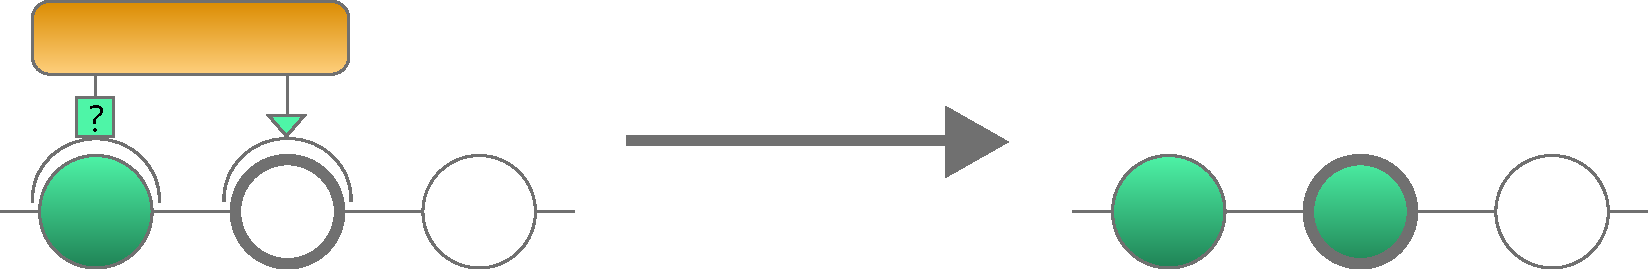
\includegraphics[width=\textwidth]{enzymes/linear_a.pdf}
                        \end{minipage}
                        \vfill
                        \begin{minipage}{0.15\textwidth}
                            \caption*{\small \textbf{(b)}}
                        \end{minipage}
                        \begin{minipage}{0.8\textwidth}
                            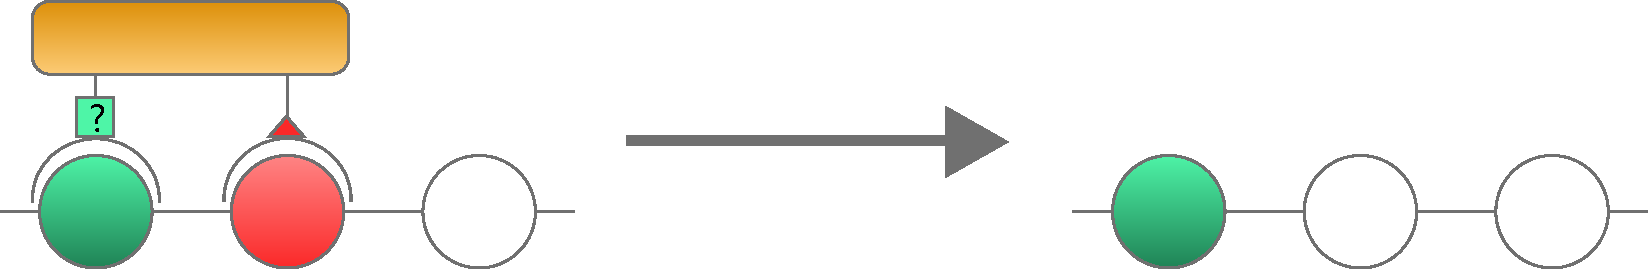
\includegraphics[width=\textwidth]{enzymes/linear_b.pdf}
                        \end{minipage}
                    \end{minipage}
                    \caption{Simplified model of linear enzyme acetylation addition \textbf{(a)} and methylation removal \textbf{(b)} reactions. Acetylated nucleosomes are coloured in green, methylated nucleosomes are red and colourless ones are unmodified. The reactions shown are also defined in the rule set to occur in the opposite direction. Linear enzymes in favour of methylation extension (or acetylation deletion) work analogically.}
                    \label{img:linearEnzymes}
                \end{figure}
                %

                %
                Linear enzymes are used to extending sites containing a specific modification (e.g. acetylation, see fig. \ref{img:linearEnzymes}) by either propagating said modification from nucleosome to neighbouring unmodified nucleosome or by deleting an opposing modification next to a nucleosome with the desired modification. They exclusively have next neighbour reach.
                %
            %
            %
            \subsubsection*{Cooperative enzymes}
                \label{subsubsec:coopEnzymes}
                %
                \begin{figure}[htpb!]
                    \centering
                    \begin{minipage}[t][3cm]{\textwidth}
                        \begin{minipage}{0.15\textwidth}
                            \caption*{\small \textbf{(a)}}
                        \end{minipage}
                        \begin{minipage}{0.8\textwidth}
                            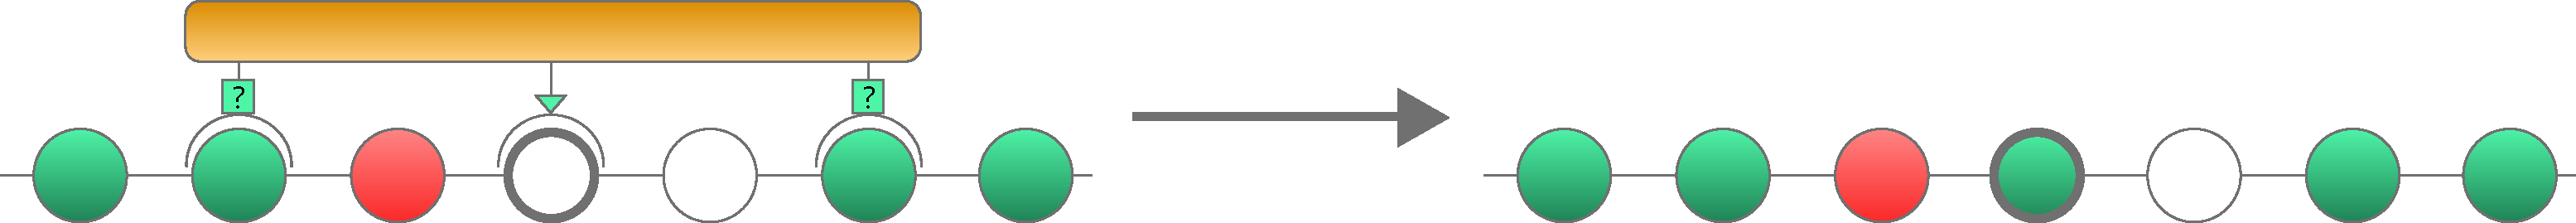
\includegraphics[width=\textwidth]{enzymes/coop_a.pdf}
                        \end{minipage}
                    \vfill
                        \begin{minipage}{0.15\textwidth}
                            \caption*{\small \textbf{(b)}}
                        \end{minipage}
                        \begin{minipage}{0.8\textwidth}
                            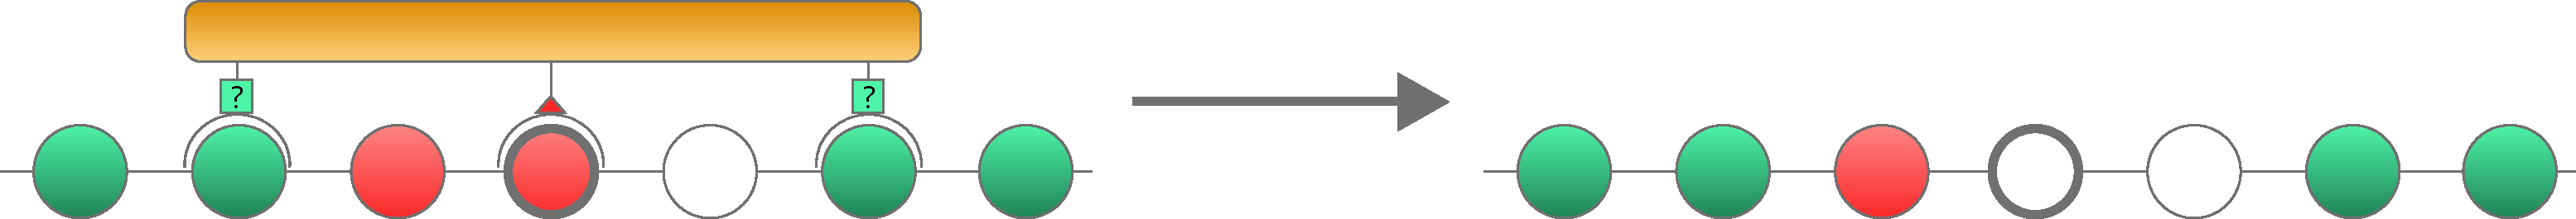
\includegraphics[width=\textwidth]{enzymes/coop_b.pdf}
                        \end{minipage}
                    \end{minipage}
                    \caption{Simplified model of cooperative enzyme acetylation addition \textbf{(a)} and methylation removal \textbf{(b)} reactions. Acetylated nucleosomes are coloured in green, methylated nucleosomes are red and colourless ones are unmodified. The reactions shown are also defined in the rule set to occur in the opposite direction. Cooperative enzyme methylation  addition and acetylation removal work analogically.}
                    \label{img:coopEnzymes}
                \end{figure}
                %

                %
                Cooperative enzymes generally read the state of two different nucleosomes on the string and write to or remove a modification from a third nucleosome. It is important to note that the two nucleosomes that are read do not need to have any next-neighbour relation to the one the enzyme is modifying.  Thus, to some extent, these enzymes, unlike any other enzyme featured in this work, take the global modification trend on the string into account: if many nucleosomes are acetylated, then cooperative enzymes in favour of acetylation (meaning cooperative acetylation adders and cooperative methylation removers) are more active which, in turn, reinforces the acetylation distribution on the string.
                %

                %
                The cooperative enzymes in this work are implemented in a way that they are always reading two nucleosomes that are equally far away from the nucleosome the enzyme wants to modify (see fig. \ref{img:coopEnzymes}).
                %

                %
                The notion of 'space' of a cooperative enzyme defines the context reach of said enzyme. For instance, a cooperative adder with a reach of 3 will read the nucleosome it wants to write on and ignore the 3 next neighbours of this nucleosome. It will only read the 4th nucleosomes situated to the left and the right of the first one. Accordingly, a cooperative enzyme which reads the next neighbours of the nucleosome to write on by definition has a reach of 0.
                %


            %
            %
            \subsubsection*{Random enzymes}
                %
                Random adder and remover enzymes serve as noise in the system. As these enzymes act on one single nucleosome, they do not take into account any other nucleosomes on the string. As such, random adders are the only enzymes featured in this work that are able to modify a nucleosome on an otherwise completely unmodified string.
                %
                \begin{figure}[htpb!]
                    \centering
                    \begin{minipage}[t][5cm]{\textwidth}
                        \begin{minipage}{0.15\textwidth}
                            \caption*{\small \textbf{(a)}}
                        \end{minipage}
                        \begin{minipage}{0.8\textwidth}
                            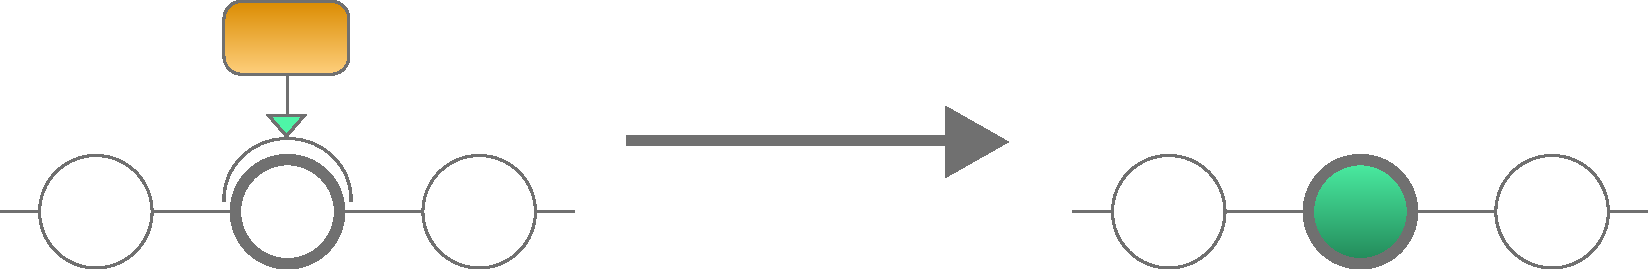
\includegraphics[width=\textwidth]{enzymes/random_a.pdf}
                        \end{minipage}
                        \vfill
                        \begin{minipage}{0.15\textwidth}
                            \caption*{\small \textbf{(b)}}
                        \end{minipage}
                        \begin{minipage}{0.8\textwidth}
                            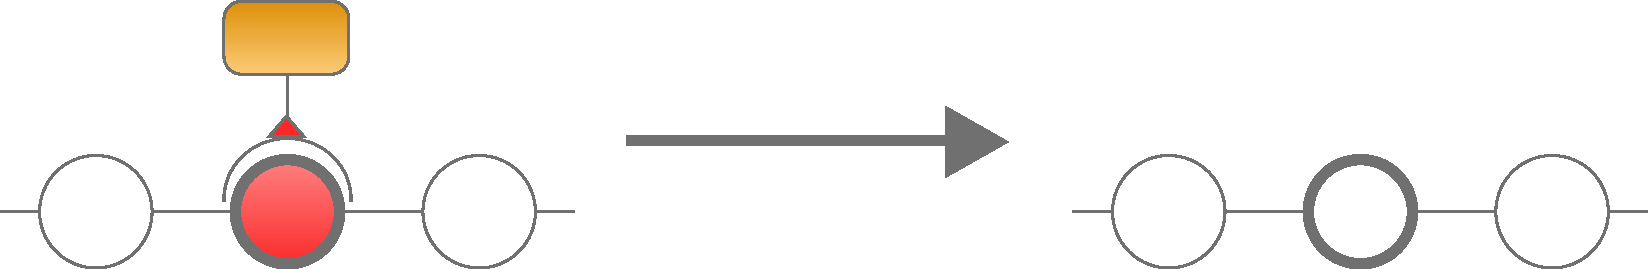
\includegraphics[width=\textwidth]{enzymes/random_b.pdf}
                        \end{minipage}
                    \end{minipage}
                    \caption{Simplified model of random enzyme acetylation addition \textbf{(a)} and methylation removal \textbf{(b)} reactions. Acetylated nucleosomes are coloured in green, methylated nucleosomes are red and colourless ones are unmodified. Random enzyme methylation addition and acetylation removal work analogically.}
                    \label{img:randomEnzymes}
                \end{figure}
                %

                %
                Random enzymes still have a context, as for example a random methylation adder cannot bind to any already modified nucleosome, only to an unmodified one. Given that any nucleosome can be targeted by a specific random enzyme at any moment, these enzymes' association rate should be smaller than the other ones' in the system by many orders of magnitude.
                %

                %
                Random enzymes are not only “enzymes” in the true sense of the word when compared to the biological side of the model. They also exist in order to mimic the “noise” that is associated with such systems.
                %

                %
                \begin{itemize}
                    {
                        \color{red}
                        \item Explain PRC2 with JARID2 DNA-binding TF subcomponent?
                    }
                \end{itemize}
                %
                %
            %
            %
            \subsubsection*{Completer enzymes}
                %
                \begin{figure}[htpb!]
                    \centering
                    \begin{minipage}[t][10cm]{\textwidth}
                        \begin{minipage}{0.15\textwidth}
                            \caption*{\small \textbf{(a)}}
                        \end{minipage}
                        \begin{minipage}{0.8\textwidth}
                            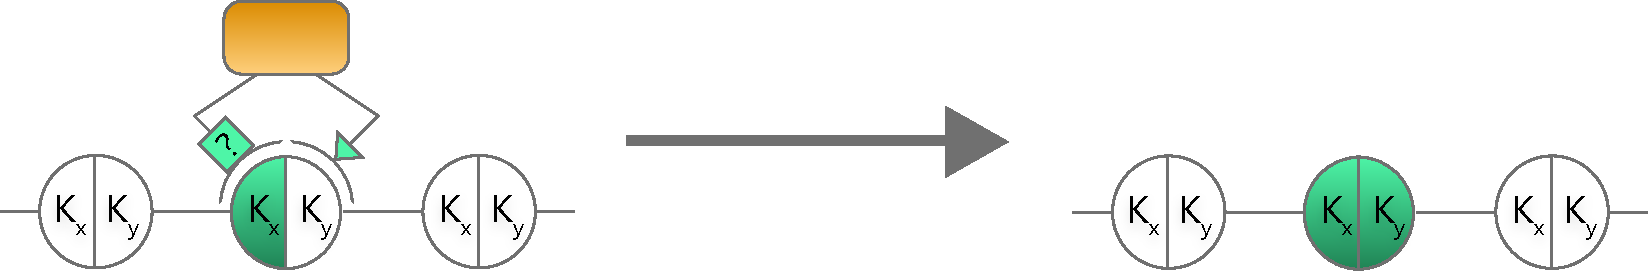
\includegraphics[width=\textwidth]{enzymes/completer_total_a.pdf}
                        \end{minipage}
                        \vfill
                        \begin{minipage}{0.15\textwidth}
                            \caption*{\small \textbf{(b)}}
                        \end{minipage}
                        \begin{minipage}{0.8\textwidth}
                            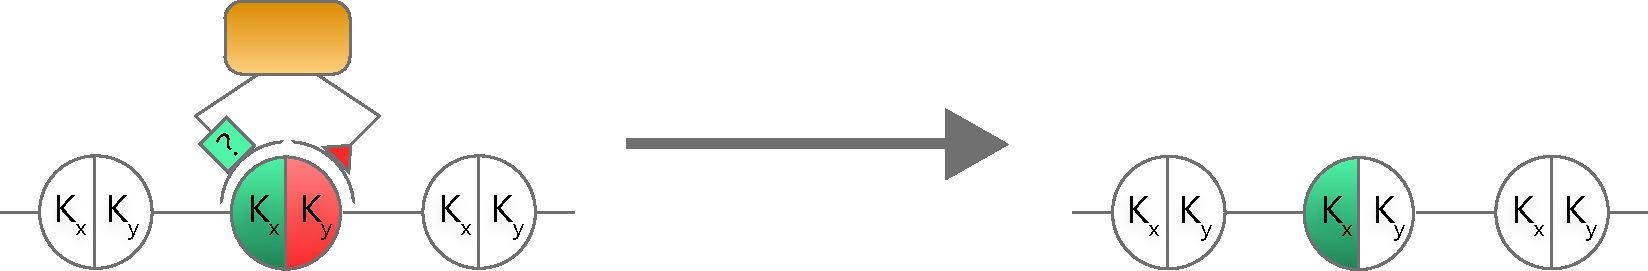
\includegraphics[width=\textwidth]{enzymes/completer_total_b.pdf}
                        \end{minipage}
                        \vfill
                        \begin{minipage}{0.15\textwidth}
                            \caption*{\small \textbf{(c)}}
                        \end{minipage}
                        \begin{minipage}{0.8\textwidth}
                            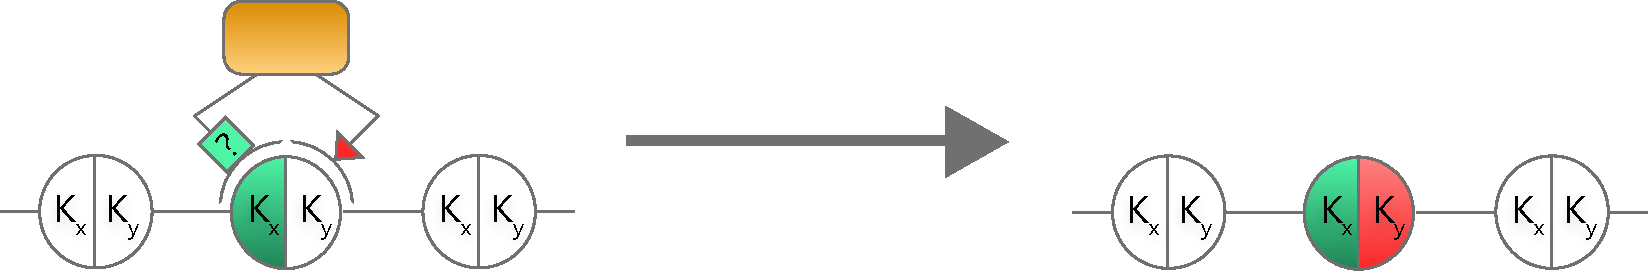
\includegraphics[width=\textwidth]{enzymes/completer_biv_a.pdf}
                        \end{minipage}
                        \vfill
                        \begin{minipage}{0.15\textwidth}
                            \caption*{\small \textbf{(d)}}
                        \end{minipage}
                        \begin{minipage}{0.8\textwidth}
                            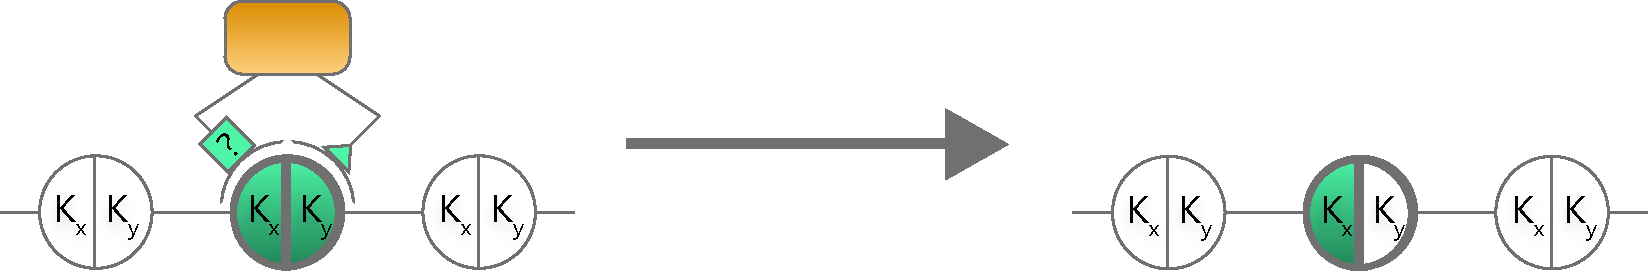
\includegraphics[width=\textwidth]{enzymes/completer_biv_b.pdf}
                        \end{minipage}
                    \end{minipage}
                    \caption{Simplified model of the enzyme acetylation addition and removal reactions. \textbf{(a)} and \textbf{(b)} show reactions in favour of “total” states, which means that they enforce one single type of modification on a nucleosome, while \textbf{(c)} and \textbf{(d)} respectively show addition and removal reactions favouring bivalent nucleosomes. The reactions shown are also defined in the rule set to occur in the opposite direction. Total enzyme methylation addition and acetylation removal work analogically.}
                    \label{img:completerEnzymes}
                \end{figure}
                %

                %
                Completer enzymes are the only enzymes featured in this work which modify two different amino acids on one single nucleosome. These amino acids are exemplarily called $K_x$ and $K_y$ and, like the amino acid on the other nucleosomes, are both methylatable and acetylatable. Completer enzymes only act on one single nucleosome. They read one amino acid and write to or remove from the other one. As such, these enzymes are used in order to reinforce the generation of bivalent states or “total” (fully acetylated or fully methylated) states among the nucleosomes.
                %

                %
                Completer enzymes have no known scientific background. They only serve the purpose of analysing the system dynamics when provoking bivalency or total states in the system.
                %
            %
            %
        %
        %
        \subsection{Enzyme rule sets}
            %
            This subsection provides an overview of the different enzyme rule sets used in the different simulations featured in this work. The rule sets are almost always kept constant throughout every section in the 'Results' chapter respectively. The enzyme rule sets used are the following (depending on the reader's preference, the rule sets can also be looked up in tab. \ref{tab:EnzymeRuleSets}):
            %

            %
            % \begin{itemize}
            %     {
            %         \item 3.1: linear adders, linear removers, random adders, random removers
            %         \item 3.2: cooperative adders, cooperative removers (not for some), random adders, random removers (non-cyclic)
            %         \item 3.3: cooperative adders, cooperative removers (not for some), random adders, random removers (cyclic)
            %         \item 3.4: cooperative adders, random adders, random removers (cyclic)
            %         \item 3.5: cooperative adders, random adders, random removers (cyclic)
            %         \item 3.6: (cyclic)
            %             \begin{itemize}
            %                 \item BivalentBistability: cooperative adders (0-5 for all), cooperative removers, random adders, random removers,
            %                 \item FavTotal: total completers, total self removers, random adders, random removers
            %                 \item FavBivalency: bivalent completers, bivalent self removers, random adders, random removers
            %             \end{itemize}
            %     }
            % \end{itemize}
            %

            %
            \begin{table}
                \centering
                \caption{Summary on whether an enzyme type was included in the designated experiment presented in the indicated 'Results' section. The \textbf{X} indicates that the enzyme type was featured, while the \textbf{~} indicates that there were some runs in this section that featured the referring enzyme type, while other runs in this same section did not. The explanation as to why this was done can be found in the respective sections.}
                \begin{tabular}{l|c|c|c|c|c|c|c|c|}
                                            & \multirow{2}{*}{3.1} & \multirow{2}{*}{3.2} & \multirow{2}{*}{3.3} & \multirow{2}{*}{3.4} & \multirow{2}{*}{3.5} & \multicolumn{3}{c|}{3.6}                        \\
                                            &                      &                      &                      &                      &                      & BivBist & Total      & Bivalent    \\\hline
                random adders               & \textbf{X}           & \textbf{X}           & \textbf{X}           & \textbf{X}           & \textbf{X}           & \textbf{X}          & \textbf{X} & \textbf{X}  \\\hline
                random removers             & \textbf{X}           & \textbf{X}           & \textbf{X}           & \textbf{X}           & \textbf{X}           & \textbf{X}          & \textbf{X} & \textbf{X}  \\\hline
                linear adders               & \textbf{X}           &                      &                      &                      &                      &                     &            &             \\\hline
                linear removers             & \textbf{X}           &                      &                      &                      &                      &                     &            &             \\\hline
                cooperative adders          &                      & \textbf{X}           & \textbf{X}           & \textbf{X}           & \textbf{X}           & \textbf{X}          &            &             \\\hline
                cooperative removers        &                      & \textbf{X}          &                       &                      &                      & \textbf{\~}         &            &             \\\hline
                bivalent completer adders   &                      &                      &                      &                      &                      &                     &            & \textbf{X}  \\\hline
                bivalent completer removers &                      &                      &                      &                      &                      &                     &            & \textbf{X}  \\\hline
                total completer adders      &                      &                      &                      &                      &                      &                     & \textbf{X} &             \\\hline
                total completer removers    &                      &                      &                      &                      &                      &                     & \textbf{X} &             \\\hline
                cyclic                      &                      &                      & \textbf{X}           & \textbf{X}           & \textbf{X}           & \textbf{X}          & \textbf{X} & \textbf{X}  \\\hline
                non-cyclic                  & \textbf{X}           & \textbf{X}           &                      &                      &                      &                     &            & \\\hline
                \end{tabular}
                \label{tab:EnzymeRuleSets}
            \end{table}
            %
        %
        %
    %
    %
    \section{Simulation details}
    \label{sec:simulationDetails}
        %
        The input files for every result section's \ed/ simulations can be found at \cite{Krecké2021}. In general, every \ed/ run needs 3 files: a \textit{statefile}, a \textit{rulefile} and a \textit{paramfile}. The \textit{statefile} contains the starting state of the nucleosome string. The \textit{rulefile} contains all specifications to the enzymes: their contexts, the modification pattern, the association rate and the dissociation rate. The \textit{paramfile} holds general information about the simulation itself with the most important one being the simulation time. This numeric parameter sets the exit condition for the algorithm.
        %

        %
        The simulation time changes significantly between some runs. This is due to Gillespie's algorithm's event-based time approach. Changing the enzyme set can result in a significantly different number of possible reactions during the simulation which can lead to very short simulation step numbers. Thus, in order to grant statistically significant runs, the simulation time was increased for certain runs, where the overall run time was empirically found to be too short.
        %

        %
        Furthermore, for reasons of performance and storage space, the graphs included in the results section were made from simulations with different simulation time. Preprocessing for the heatmaps was significantly more expensive than the other plots. Therefore, heatmaps were generated from \textit{short} runs, whereas the other plots were generated from \textit{long} runs. Meaning:
        %

        %
        \begin{itemize}
            \item \textit{short}: Every step (event) is plotted and metadata are used to plot association numbers and relative binding time (resulting in heatmaps).
            \item \textit{long}: Only every 1000th step is plotted. Given that the system is chaotic thanks to the random nature of the algorithm, regular plotting (f. ex. every 1000th data point) results in a smoothing of the histogram because the chosen data points are more representative for the underlying distribution.
        \end{itemize}
        %

        %
        The different simulation parameters for the runs featured in this work are summarized in \ref{tab:simulationParametersSummary}.
        %
    %
    %
%
%